\documentclass[article,shortnames]{jss}

%% -- LaTeX packages and custom commands ---------------------------------------

%% recommended packages
\usepackage{orcidlink,thumbpdf,lmodern}

%% additional packages
\usepackage{amssymb,amsmath}

%% new custom commands
\newcommand{\class}[1]{`\code{#1}'}
\newcommand{\fct}[1]{\code{#1()}}

%% For Sweave-based articles about R packages:
%% need no \usepackage{Sweave}


%% -- Article metainformation (author, title, ...) -----------------------------

%% - \author{} with primary affiliation
%% - \Plainauthor{} without affiliations
%% - Separate authors by \And or \AND (in \author) or by comma (in \Plainauthor).
%% - \AND starts a new line, \And does not.
\author{Lennart Oelschl\"ager~\orcidlink{0000-0001-5421-9313}\\Bielefeld University \And Dietmar Bauer~\orcidlink{0000-0003-2920-7032}\\Bielefeld University}
\Plainauthor{Lennart Oelschl\"ager, Dietmar Bauer}

%% - \title{} in title case
%% - \Plaintitle{} without LaTeX markup (if any)
%% - \Shorttitle{} with LaTeX markup (if any), used as running title
\title{\pkg{RprobitB}: Bayes Estimation of Choice Behavior Heterogeneity in \proglang{R}}
\Plaintitle{RprobitB: Bayes Estimation of Choice Behavior Heterogeneity in R}
\Shorttitle{\pkg{RprobitB}}

%% - \Abstract{} almost as usual
\Abstract{
\pkg{RprobitB} is an \proglang{R} package for Bayes estimation of probit choice models, both in the cross-sectional and panel setting. The package can analyze binary, multivariate, ordered, and ranked choices, and places a special focus on modeling heterogeneity of choice behavior among deciders. The main functionality includes model fitting via Markov chain Monte Carlo methods, tools for convergence diagnostic, choice data simulation, in-sample and out-of-sample choice prediction, and model selection using information criteria and Bayes factors. The latent class model extension facilitates preference-based decider classification, where the number of latent classes can be inferred via the Dirichlet process or a weight-based updating scheme. This allows for flexible modeling of choice behavior without the need to impose structural constraints on the form of the heterogeneity. To demonstrate the application of the method, we reveal three different playing strategies of participants in an online chess tournament, where each chess player can be assigned a probability of following each of the strategies.
}

%% - \Keywords{} with LaTeX markup, at least one required
%% - \Plainkeywords{} without LaTeX markup (if necessary)
%% - Should be comma-separated and in sentence case.
\Keywords{discrete choice, probit model, choice behavior heterogeneity, Bayes estimation, decider classification, \proglang{R}}
\Plainkeywords{discrete choice, probit model, choice behavior heterogeneity, Bayes estimation, decider classification, R}

%% - \Address{} of at least one author
%% - May contain multiple affiliations for each author
%%   (in extra lines, separated by \emph{and}\\).
%% - May contain multiple authors for the same affiliation
%%   (in the same first line, separated by comma).
\Address{
  Lennart Oelschl\"ager, Dietmar Bauer\\
  Department of Business Administration and Economics\\
  Bielefeld University\\
  Postfach 10 01 31, Germany\\
  E-mail: \email{lennart.oelschlaeger@uni-bielefeld.de}, \email{dietmar.bauer@uni-bielefeld.de}
}

\begin{document}

%% -- Introduction -------------------------------------------------------------

%% - In principle "as usual".
%% - But should typically have some discussion of both _software_ and _methods_.
%% - Use \proglang{}, \pkg{}, \fct{} and \code{} markup throughout the manuscript.
%% - If such markup is in (sub)section titles, a plain text version has to be
%%   added as well.
%% - All software mentioned should be properly \cite-d.
%% - All abbreviations should be introduced.
%% - Unless the expansions of abbreviations are proper names (like "Journal
%%   of Statistical Software" above) they should be in sentence case (like
%%   "generalized linear models" below).

\section{Introduction}
\label{sec:introduction}

Discrete choice models aim to explain past and predict future choice behavior. They do so by connecting observed choices to observed covariates that influence the decision, such as attributes of the choice alternatives or decider's socio-demographic characteristics. While some influencing characteristics are easily measurable through surveys (like income and household size), others are not. For example, the preference for a low-emission car versus an SUV powered by a combustion engine will be influenced by the environmental concerns. The political attitude of the car buyer is hard to quantify, so it is typically not queried. But not accounting for such unobserved choice behavior heterogeneity generally leads to an inferior model fit. The \proglang{R} \citep{R} package \pkg{RprobitB}\footnote{The package name is a portmanteau of the language \proglang{R}, the probit model, and the Bayes framework.} \citep{Oelschlaeger:2022} implements state-of-the-art tools for modeling taste heterogeneity in the context of discrete choices.

Discrete choice models are commonly interpreted as random utility models. This model class assumes that the deciders obtain utility values for the available alternatives which they seek to maximize. The utilities are unobserved by the researcher and hence modeled by a function of the covariates, in our case a linear combination of those, and a random error term. The error term distribution determines the model type, where \pkg{RprobitB} implements the probit model, assuming a joint normal distribution across alternatives (as opposed, e.g., to the logit model which assumes independent extreme value distributions). The coefficients of the linear combination represent the ceteris paribus effect of the covariates on the utility, and ratios of coefficients quantify substitution patterns, for example the willingness to pay more money for a lower CO2 emission rate.

Constant coefficients across deciders result in substitution patterns that again are constant. This can be unreasonable in certain scenarios, including the car purchase example from above. In such cases, explicit modeling of the decider's preferences would be preferable but limited by data availability. In the panel data case with many observations for each decider, fixed effect models provide options. For short panels or in cross-sectional data sets, the random effect model is a remedy, where the coefficients are assumed to be stemming from a multivariate normal (mixing) distribution. This specification allows for decider-specific coefficients and characterizes the taste heterogeneity, cf., \cite{Train:2009} and \cite{Bhat:2011}. Some applications require even more flexibility: the empirical study \cite{Cirillo:2006} for example fits a bi-modal distribution to the values of travel time savings. For such cases, \pkg{RprobitB} provides the recently proposed approach of \cite{Oelschlaeger:2020} that approximates any underlying mixing distributions by a mixture of Gaussian densities, leading to the latent class mixed probit model.

The latent class model extension also enables preference-based decider classification, i.e., identifying groups of deciders with similar preferences. This requires a reasonable specification of the total class number. While a trial-and-error strategy in conjunction with likelihood-based model selection is theoretically possible, \pkg{RprobitB} offers two data-driven approaches that avoid the need to pre-specify the class number: weight-based class updates within the estimation routine \citep{Oelschlaeger:2020} and class updates based on the Dirichlet process, similar to \cite{Burda:2008}.

\pkg{RprobitB} implements Bayesian estimation via Markov chain Monte Carlo simulation, which has several benefits compared to the frequentist alternative for latent class mixed probit models: it does not need to compute the probit likelihood (which is not in closed form and hence would require approximation), it avoids numerical challenges associated with finding the likelihood optimum, it enables to impose prior believes on the model parameters, and it provides posterior parameter distributions instead of point estimates only. Additionally, the Bayesian approach was shown to be computationally faster with increasing number of random effects and normal mixing distributions than the maximum likelihood approach, cf., \cite{Train:2001} for a simulation study in the logit case.

There already exist several open-source implementations for discrete choice modeling: \pkg{Rchoice} \citep{Sarrias:2016} and \pkg{mlogit} \citep{Croissant:2020} are two \proglang{R} packages for maximum likelihood estimation (MLE) of the (mixed) probit and logit model. The \proglang{Python} \citep{Python} library \pkg{Biogeme} \citep{Bierlaire:2020} can additionally estimate latent class (LC) models. In \proglang{Julia} \citep{Julia}, the \pkg{DiscreteChoiceModels.jl} package \citep{Bhagat:2022} currently only supports the multinomial logit model. The \proglang{R} package \pkg{gmnl} \citep{Sarrias:2017} provides generalized and latent class mixed multinomial logit models, while the \pkg{apollo} package \citep{Hess:2019} allows for more flexible logit and probit model specifications, with both maximum likelihood and Bayesian estimation. The \proglang{R} packages \pkg{bayesm} \citep{Rossi:2019} and \pkg{MNP} \citep{Imai:2022} are two alternatives for Bayesian estimation of the probit model, both implementing Markov chain Monte Carlo simulation methods similar to \pkg{RprobitB}. The \pkg{RprobitB} package complements this collection by implementing latent class mixed probit models in conjunction with class updating schemes, as outlined above. The software comparison is summarized in Table \ref{tab:pkg_overview}.

\begin{table}[!ht]
\centering
\begin{tabular}{l|ccccccc}
                              & Probit      & Logit      & Bayes      & MLE        & Mixed      & LC           & LC update  \\ \hline
\pkg{Rchoice}                 & \checkmark  & \checkmark &            & \checkmark & \checkmark &              &            \\
\pkg{mlogit}                  & \checkmark  & \checkmark &            & \checkmark & \checkmark &              &            \\
\pkg{Biogeme}                 & \checkmark  & \checkmark &            & \checkmark & \checkmark & \checkmark   &            \\
\pkg{DiscreteChoiceModels.jl} &             & \checkmark &            & \checkmark &            &              &            \\
\pkg{gmnl}                    &             & \checkmark &            & \checkmark & \checkmark & \checkmark   &            \\
\pkg{apollo}                  & \checkmark  & \checkmark & \checkmark & \checkmark & \checkmark & \checkmark   &            \\
\pkg{bayesm}                  & \checkmark  & \checkmark & \checkmark &            & \checkmark &              &            \\
\pkg{MNP}                     & \checkmark  &            & \checkmark &            &            &              &            \\
\pkg{RprobitB}                & \checkmark  &            & \checkmark &            & \checkmark & \checkmark   & \checkmark \\
\end{tabular}
\label{tab:pkg_overview}
\caption{Overview of open-source software for estimating discrete choice models.}
\end{table}

% Article overview
This article provides a general description of choice modeling with \pkg{RprobitB} and is structured as follows. To fix our notation, Section \ref{sec:probit_model} defines the probit model and formalizes the concepts of mixing distributions and latent classes. Sections \ref{sec:choice_data} to \ref{sec:model_selection} describe the package workflow, including choice data preparation, simulation, model fitting, choice prediction, preference classification, and model selection. The main functions for these tasks are visualized in the flowchart Figure \ref{fig:flowchart}. We illustrate the functions throughout the paper using three different real world data sets: the two stated-choice data sets \code{Train} and \code{Electricity} from \pkg{mlogit} allow for result comparison across packages and between the probit and logit model class, while we use a revealed-choice data set about online chess strategy (that is contained in \pkg{RprobitB}) to demonstrate flexible preference classification using the Dirichlet process. A simulation example demonstrates the accuracy of the model parameter estimates. Section \ref{sec:conclusion} concludes and gives an outlook of anticipated package extensions.

\begin{figure}[!ht]
  \centering
  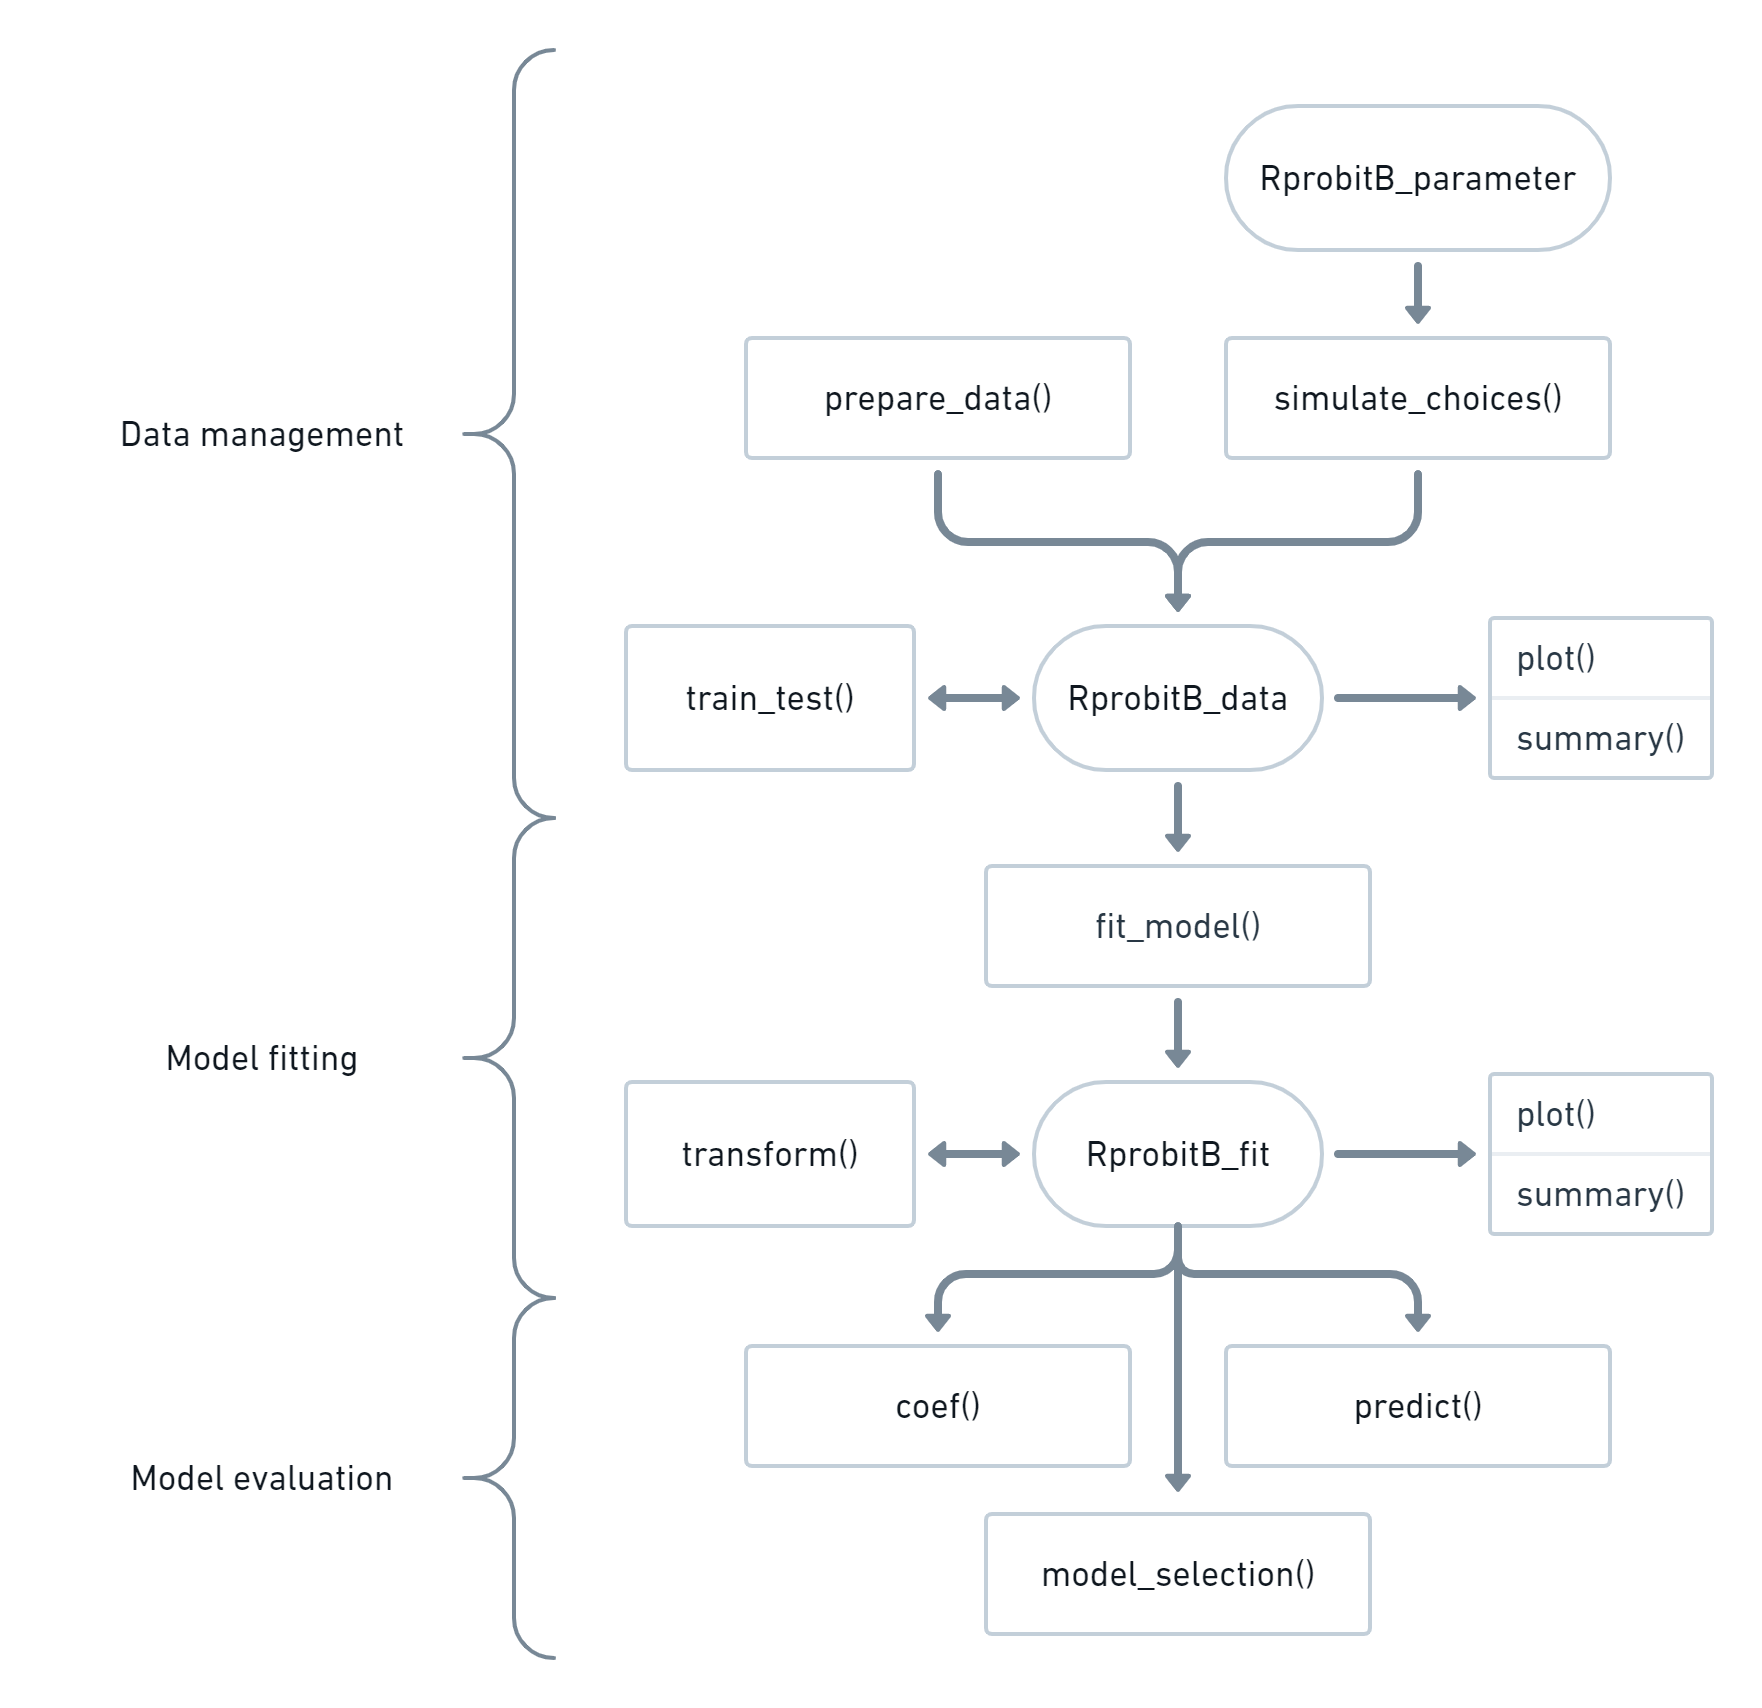
\includegraphics[width=1.0\textwidth]{flowchart.png}
  \caption{Flowchart of the main \pkg{RprobitB} functionalities (rectangles) and objects (ovals).}
  \label{fig:flowchart}
\end{figure}

\section{The probit model} \label{sec:probit_model}

Assume that we know the choices of $N$ deciders choosing between $J \geq 2$ alternatives at each of $T$ choice occasions.\footnote{The number $T$ of choice occasions is the same for each decider here for notational simplicity. However, \pkg{RprobitB} allows for unbalanced panels, i.e., varying $T$. Of course, the cross-sectional case $T = 1$ is possible.} Specific to each decider, alternative and choice occasion, we observe $P$ covariates, a linear combination of which eventually explains the latent random utility:
%
\begin{equation}
  \label{eq:utility}
  U_{ntj} = X_{ntj}^\top \tilde{\beta}_n + \epsilon_{ntj}
\end{equation}
%
for $n=1,\dots,N$, $t=1,\dots,T$ and $j=1,\dots,J$. Here, $X_{ntj}$ is a (column) vector of $P$ characteristics specific to alternative $j$ as faced by decider $n$ at choice occasion $t$, $\tilde{\beta}_n \in \mathbb{R}^{P}$ is the coefficient vector encoding the preferences of $n$, and $(\epsilon_{nt:}) = (\epsilon_{nt1},\dots,\epsilon_{ntJ})^\top \sim \text{MVN}_{J} (0,\Sigma)$ is the model's error term vector for $n$ at $t$.

The value $U_{ntj}$ on the left-hand side of equation Equation~\ref{eq:utility} can be interpreted as the decider's utility. It is unobserved by the researcher, but we assume that the deciders know their utilities for each alternative and make a choice which is consistent with utility maximization.\footnote{Utility maximizing behavior is a common assumption in econometric models. However, studies have shown that humans do not always decide in this rational sense \citep{Tversky:1986, Hewig:2011}. See also \citep{Thaler:2015} for a survey of the history of the discipline of behavioral economics.} Therefore,
%
\begin{equation}
   \label{eq:link}
   y_{nt} = \operatorname*{argmax}_{j = 1,\dots,J} U_{ntj},
\end{equation}
%
where $y_{nt}=j$ denotes the event that decider $n$ chooses $j$ at her $t$-th choice occasion.

Equation~\ref{eq:utility} has a decider-specific coefficient vector $\tilde{\beta}_n$. Some entries of $\tilde{\beta}_n$ can be fixed across deciders, in which case the coefficient vector is of the form $\tilde{\beta}_n^\top = (\alpha^\top, \beta_n^\top)^\top$, where $\alpha \in \mathbb{R}^{P_f}$ are $P_f$ coefficients that are constant across deciders and $\beta_n$ are $P_r$ decider-specific coefficients, $P_f + P_r = P$. The decider-specific coefficients are assumed to be realizations of an underlying mixing distribution. This distribution characterizes heterogeneity among the deciders and allows for individual sensitivities as motivated in the introduction.

Choosing an appropriate mixing distribution is a notoriously difficult task of the model specification. In many applications, different types of standard parametric distributions (including the normal, log-normal, uniform and tent distribution) are tried in conjunction with a likelihood value-based model selection \citep[pp.\ 136 ff.]{Train:2009}. Instead, \pkg{RprobitB} implements the approach of \cite{Oelschlaeger:2020} to approximate any underlying mixing distribution by a mixture of $P_r$-variate Gaussian densities $\phi_{P_r}$ with mean vectors $b=(b_c)_{c}$ and covariance matrices $\Omega=(\Omega_c)_{c}$ using $C$ components:
%
\begin{align*}
\beta_n\mid b,\Omega \sim \sum_{c=1}^{C} s_c \phi_{P_r} (\cdot \mid b_c,\Omega_c).
\end{align*}
%
Here, $(s_c)_{c}$ are weights satisfying $0 < s_c\leq 1$ for $c=1,\dots,C$ and $\sum_c s_c=1$. One interpretation of the latent class model is obtained by introducing variables $z=(z_n)_n$, allocating each decision maker $n$ to class $c$ with probability $s_c$, i.e.,
%
\begin{align*}
\text{Prob}(z_n=c)=s_c \land \beta_n \mid z,b,\Omega \sim \phi_{P_r}(\cdot \mid b_{z_n},\Omega_{z_n}).
\end{align*}
%
This interpretation allows for decider classifications, see Section \ref{subsec:dp_update} for an example.

Finally, the probit model requires normalization, because any utility model is invariant towards the level and the scale of utility \citep[Ch.\ 2]{Train:2009}. We therefore normalize the model by taking differences in Equation~\ref{eq:utility} and fixing one error term variance:
%
\begin{equation}
\label{eq:utility_diff}
\tilde{U}_{ntj} = \tilde{X}_{ntj}^\top \tilde{\beta}_n + \tilde{\epsilon}_{ntj},
\end{equation}
%
where (choosing some alternative $k \in \{1,\dots,J\}$ as the reference) $\tilde{U}_{ntj} = U_{ntj} - U_{ntk}$, $\tilde{X}_{ntj} = X_{ntj} - X_{ntk}$, and $\tilde{\epsilon}_{ntj} = \epsilon_{ntj} - \epsilon_{ntk}$ for $j\neq k$. The error term differences $(\tilde{\epsilon}_{nt:})$ again are multivariate normally distributed with mean 0 but transformed covariance matrix $\tilde{\Sigma}$, in which we fix one diagonal element to a positive number.\footnote{Fixing one element of $\tilde{\Sigma}$ determines the utility scale. Fixing one fixed effect (i.e., one entry of $\alpha$) serves the same purpose. Both alternatives are implemented, see Section \ref{subsec:estimation_routine}.}

\section{Choice data} \label{sec:choice_data}

\pkg{RprobitB} requests that choice data sets are a) of class \class{data.frame}, b) in wide format (i.e., each row provides the full information for one choice occasion), c) contain a column with unique identifiers for each decision maker (and optionally each choice occasion), d) contain a column with the observed choices (required for model fitting but not for prediction), and e) contain columns for the values of (alternative and/or decider specific) covariates. The underlying set of choice alternatives is assumed to be mutually exclusive (one can choose one and only one alternative that are all different), exhaustive (the alternatives do not leave other options open), and finite \citep[Ch.\ 2]{Train:2009}. Alternatives can be considered as ordered (e.g., the level of agreement on a Likert rating scale), and additionally full rankings of the alternatives can be provided (e.g., when asking the respondent to rank all available alternatives from best to worst).

\subsection{Different types of covariates} \label{subsec:covariate_types}

Different covariate types can be considered: covariates that are constant across alternatives (e.g., a car buyer's income), covariates that are alternative specific (e.g., the car's price), covariates with the same coefficient for all alternatives (e.g., the car price may have the same impact on all alternatives), and covariates that have alternative specific coefficients (e.g., the range of an electric car might be of more importance than for other types of propulsion). To allow for these different types, we generalize Equation~\ref{eq:utility} to
%
\begin{align}
  \label{eq:utility_gen}
  U_{ntj} = \beta_{0j} + A_{ntj} \beta_1 + B_{nt} \beta_{2j} + C_{ntj} \beta_{3j} + \epsilon_{ntj}.
\end{align}
%
Here, the covariates $A$ and $C$ depend on the alternative $j$, while $B$ is only decider and choice occasion specific. The coefficient $\beta_1$ for $A$ is constant (i.e., the same for each alternative), whereas $\beta_{2j}$ and $\beta_{3j}$ for $B$ and $C$ are alternative specific. The intercepts $\beta_0j$ are called alternative specific constants (ASCs). ASCs capture the average effect on the alternative's utility of all factors that are not included in the model.

Note that the full collections $(\beta_{0j})_{j=1,\dots,J}$ of ASCs and $(\beta_{2j})_{j=1,\dots,J}$ of coefficients for covariate type $B$ are not identified. This is because we took utility differences for model normalization (cf., Section \ref{sec:probit_model}), and hence one coefficient is a linear combination of the others, respectively. To achieve identifiability, we fix $\beta_{0k}$ and $\beta_{2k}$ to 0 for one base alternative $k$. The coefficients $(\beta_{0j})_{j\neq k}$ and $(\beta_{2j})_{j\neq k}$ then have to be interpreted with respect to $k$.

\subsection{Formula framework} \label{subsec:formula}

Specifying Equation~\ref{eq:utility_gen} in \proglang{R} requires a flexible formula framework. \pkg{RprobitB} can interpret a \class{formula} object of the form \code{choice ~ A | B | C}, where \code{choice} is the name of the dependent variable (the discrete choice we aim to explain), and \code{A}, \code{B}, and \code{C} are the different covariate types of Section \ref{subsec:covariate_types}.\footnote{We adapted this formula framework from the \pkg{mlogit} package.}

The framework has the following rules. ASCs are added to the model by default. They can be removed by adding \code{+0} in the second spot, e.g., \code{choice ~ A | B + 0 | C}. To exclude covariates of the backmost categories, use either \code{0}, e.g., \code{choice ~ A | B | 0} or just leave this part out and write \code{choice ~ A | B}. However, to exclude covariates of front categories, we have to use \code{0}, e.g., \code{choice ~ 0 | B}. To include more than one covariate of the same category, use \code{+}, e.g., \code{choice ~ A1 + A2 | B}. If we don't want to include any covariates of the second category but want to estimate ASCs, add \code{1} in the second spot, e.g., \code{choice ~ A | 1 | C}. The expression \code{choice ~ A | 0 | C} is interpreted as no covariates of the second category and no alternative specific constants.

\subsection{Preparing data for estimation} \label{subsec:prepare_data}

Before model estimation, any \code{choice\_data} set must pass the \fct{prepare\_data} function together with a formula object \code{form} introduced in Section \ref{subsec:formula}:

\begin{Schunk}
\begin{Sinput}
> prepare_data(form = form, choice_data = choice_data)
\end{Sinput}
\end{Schunk}

The function performs compatibility checks and data transformations, and returns an object of class \class{RprobitB\_data} that can be fed into the estimation routine \fct{fit\_model} (that we introduce in Section \ref{subsec:estimation_routine}). The following arguments of \fct{prepare\_data} are optional:
\begin{itemize}
  \item \code{re}: A character vector of covariate names in \code{form} with random effects. Per default \code{re = NULL}, i.e., no random effects.
  \item \code{alternatives}: A character vector of the alternative names, defining the choice set. If not specified, all chosen alternatives in \code{choice\_data} are considered.
  \item \code{ordered} and \code{ranked}: Two booleans, that are set to \code{FALSE} by default. If set to \code{TRUE}, the alternatives are interpreted as ordered, or the choices are interpreted as ranked, respectively.
  \item \code{base}: One element of \code{alternatives} specifying the base alternative (cf., Section \ref{subsec:covariate_types}). Per default, \code{base} is the last element of \code{alternatives}.
  \item \code{id} and \code{idc}: The names of the columns in \code{choice_data} that contain unique identifier for each decision maker and for each choice occasion, respectively. Per default, \code{id = "id"} and \code{idc = NULL}, in which case the choice occasion identifier are generated by the appearance of the choices in the \code{choice\_data}.
  \item \code{standardize}: A character vector of variable names of \code{form} that get standardized, i.e., rescaled to have a mean of 0 and a standard deviation of 1 (none by default).
  \item \code{impute}: A character, specifying how to handle missing covariates in \code{choice\_data}. Options are \code{"complete\_cases"} (removing rows that contain missing entries, which is the default behavior), \code{"zero"} (replacing missing entries by 0), and \code{"mean"} (imputing missing entries by the covariate mean).
\end{itemize}

\paragraph{Example 1: Train trips.}

The \pkg{mlogit} package contains the data set \code{Train} with 2929 stated choices of 235 deciders between two fictional train trip alternatives \code{A} and \code{B}. The trip alternatives are characterized by their \code{price}, the travel \code{time}, the level of \code{comfort} (the lower the value the higher the comfort), and the number of \code{change}s. The data is in wide format; the columns \code{id} and \code{choiceid} identify the deciders and the choice occasions, respectively; the column \code{choice} provides the choices. For convenience, we transform \code{time} from minutes to hours and \code{price} from Dutch guilders to euros:

\begin{Schunk}
\begin{Sinput}
> data("Train", package = "mlogit")
> Train$price_A <- Train$price_A / 100 * 2.20371
> Train$price_B <- Train$price_B / 100 * 2.20371
> Train$time_A <- Train$time_A / 60
> Train$time_B <- Train$time_B / 60
> str(Train)
\end{Sinput}
\begin{Soutput}
'data.frame':	2929 obs. of  11 variables:
 $ id       : int  1 1 1 1 1 1 1 1 1 1 ...
 $ choiceid : int  1 2 3 4 5 6 7 8 9 10 ...
 $ choice   : Factor w/ 2 levels "A","B": 1 1 1 2 2 2 2 2 1 1 ...
 $ price_A  : num  52.9 52.9 52.9 88.1 52.9 ...
 $ time_A   : num  2.5 2.5 1.92 2.17 2.5 ...
 $ change_A : num  0 0 0 0 0 0 0 0 0 0 ...
 $ comfort_A: num  1 1 1 1 1 0 1 1 0 1 ...
 $ price_B  : num  88.1 70.5 88.1 70.5 70.5 ...
 $ time_B   : num  2.5 2.17 1.92 2.5 2.5 ...
 $ change_B : num  0 0 0 0 0 0 0 0 0 0 ...
 $ comfort_B: num  1 1 0 0 0 0 1 0 1 0 ...
\end{Soutput}
\end{Schunk}

For demonstration, we include all choice characteristics into our probit model, connect them to constant and fixed coefficients, and exclude ASCs:

\begin{Schunk}
\begin{Sinput}
> form <- choice ~ price + time + comfort + change | 0
\end{Sinput}
\end{Schunk}

Passing \code{form} to \fct{prepare\_data} returns an \class{RprobitB\_data} object. We will feed this object into the estimation routine \fct{fit\_model} in Section \ref{sec:model_fitting}.

\begin{Schunk}
\begin{Sinput}
> data_train <- prepare_data(
+    form = form, choice_data = Train, id = "id", idc = "choiceid"
+  )
\end{Sinput}
\end{Schunk}

The \fct{summary} and \fct{plot} methods are useful for a first data overview:

\begin{Schunk}
\begin{Sinput}
> summary(data_train)
\end{Sinput}
\begin{Soutput}
                 count
deciders           235
choice occasions  5-19
total choices     2929
alternatives         2
- 'A'             1474
- 'B'             1455
\end{Soutput}
\end{Schunk}

\begin{Schunk}
\begin{Sinput}
> plot(data_train)
\end{Sinput}
\end{Schunk}
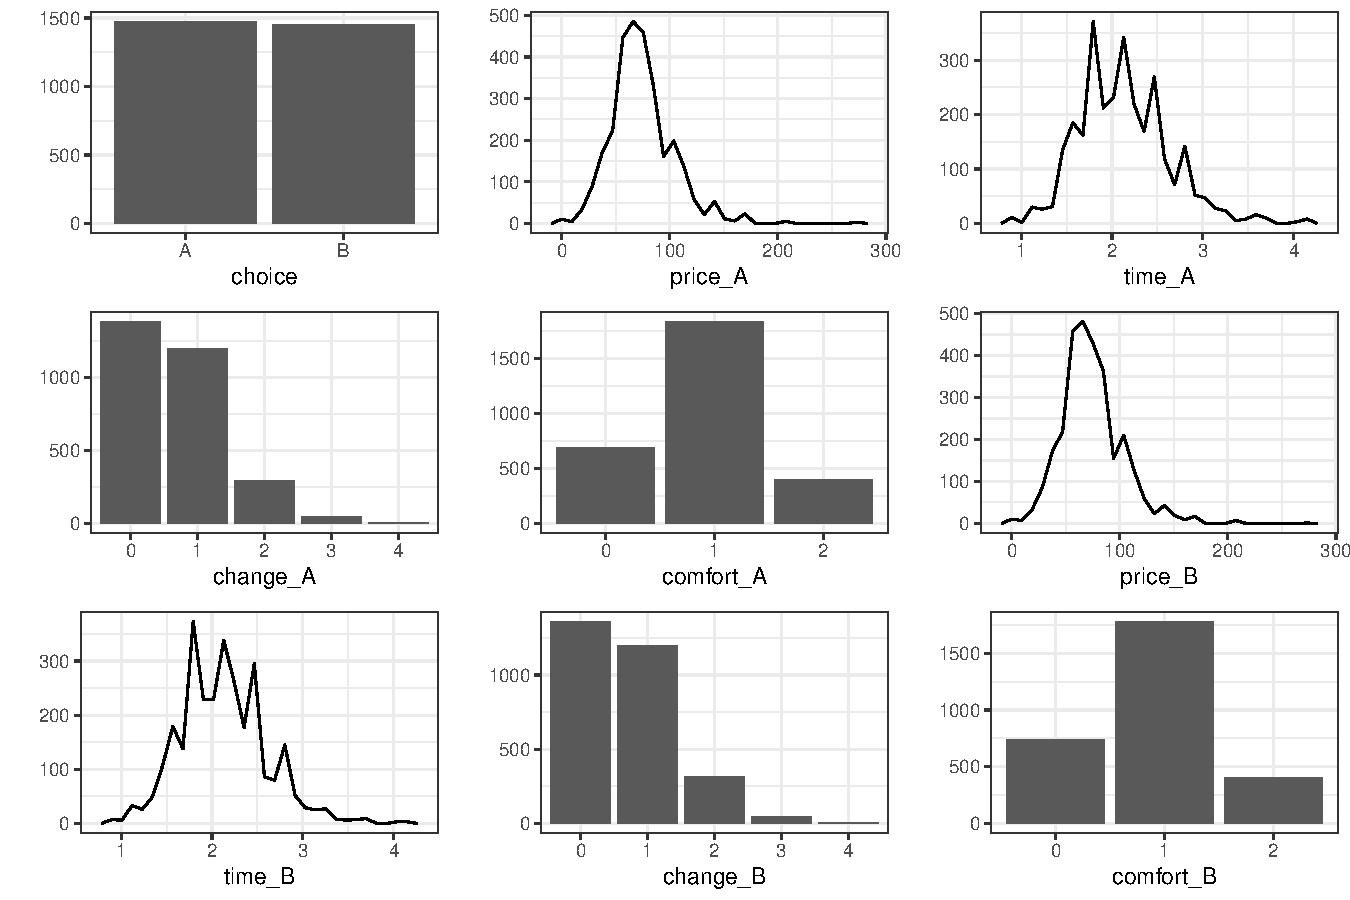
\includegraphics{rprobitb_oelschlaeger_bauer-train-data}

\subsection{Ordered alternatives} \label{subsec:ordered_alternatives}

The two choice alternatives from the train trip example are unordered. If we had asked "rate your train trip from 1 (horrible) to 7 (great)", then the respondents would choose from a set of ordered alternatives. Such ordered alternatives can by analyzed by setting \code{ordered = TRUE} in \fct{prepare\_data}. In this case, \code{alternatives} becomes a mandatory argument, where the alternatives must be named from worst to best.

Deciders obtaining separate utilities for each alternative is no longer a natural concept in this case \citep[Ch.\ 7.4]{Train:2009}. Instead, we model only a single utility
%
\begin{align*}
  U_{nt} = X_{nt}^\top \beta_n + \epsilon_{nt}
\end{align*}
%
per decider $n$ and choice occasion $t$. The value can be interpreted as the level of association that $n$ has with the choice question. It falls into discrete categories, which in turn are linked to the ordered alternatives $j=1,\dots,J$. Formally, we replace the link in Equation~\ref{eq:link} by
%
\begin{align*}
   y_{nt} = \sum_{j = 1,\dots,J} j \cdot I(\gamma_{j-1} < U_{nt} \leq \gamma_{j}),
\end{align*}
%
where $\gamma_0 = -\infty$ and $\gamma_J = +\infty$. This implies that alternative $j$ is chosen, if the utility falls into the interval $(\gamma_{j-1}, \gamma_j]$. Monotonicity of the thresholds $(\gamma_j)_{j=1,\dots,J-1}$ is ensured by estimating logarithmic increments $d_j$ with $\gamma_j = \sum_{i\leq j} \exp{(d_i)}$, $j=1,\dots,J-1$. For level normalization, we fix $\gamma_1 = 0$.

\subsection{Ranked choices} \label{subsec:ranked_choices}

Ranked choices are yet another model variation: rather than recording only the single most preferred alternative, some surveys ask for a full ranking of all the alternatives, which reveals far more about the underlying preferences. Ranked choices can by analyzed by setting \code{ranked = TRUE} in \fct{prepare\_data}. The choice column of the data set must provide the full ranking for each choice occasion (from most preferred to least preferred), where the alternatives are separated by commas, see \code{help(prepare\_data, package = "RprobitB")} for details.

The ranked probit model follows directly from the general unordered case noting that the ranking implies that the highest ranked alternative is chosen in any case, while the second highest ranked alternative is chosen, if the highest ranked alternative is not available and so forth. The only difference is that we take flexible utility differences such that the differenced utility vector is always negative, in contrast to Equation~\ref{eq:utility_diff} where we differenced with respect to a fixed reference alternative. Thereby, we incorporate information of the full ranking \citep[Ch.\ 7.3]{Train:2009}.

\subsection{Simulating choice data} \label{subsec:simulate_choice_data}

Simulation typically serves to assess the properties of the estimation algorithm either for research or in a bootstrap like fashion. The \fct{simulate\_choices} function simulates choice data from a prespecified probit model. In order to simulate the choices of \code{N} deciders in \code{T} choice occasions\footnote{\code{T} can be either a single integer for a fixed number of choice occasions per decider, or a vector of length \code{N} with decision maker specific numbers of choice occasions.} among \code{J} alternatives, we call

\begin{Schunk}
\begin{Sinput}
> simulate_choices(form = form, N = N, T = T, J = J)
\end{Sinput}
\end{Schunk}

where \code{form} is a model formula (cf., Section \ref{subsec:formula}). The following arguments are optional:
\begin{itemize}
  \item \code{re}, \code{ordered}, \code{ranked}, \code{base}, \code{standardize}: Analogue to \fct{prepare\_data}.
  \item \code{alternatives}: A character vector of length \code{J} with the names of the choice alternatives (by default the first \code{J} uppercase letters of the Roman alphabet).
  \item \code{covariates}: A named list of covariate values. Each element must be a vector of length equal to the number of choice occasions and named according to a covariate. Unspecified covariates are drawn from a standard normal distribution.
  \item \code{seed}: Optionally set a seed for the simulation.
\end{itemize}

The model parameters are set at random by default. Alternatively, they can be specified via a named list for the function's \code{true\_parameter} argument. The list can contain
\begin{itemize}
  \item a numeric vector \code{alpha} with fixed effects,
  \item the number \code{C} of latent classes (\code{C = 1} by default),
  \item a numeric vector \code{s} of length \code{C} with class weights,
  \item a matrix \code{b} with class means as columns,
  \item a matrix \code{Omega} with vectorized class covariance matrices as columns,
  \item a matrix \code{Sigma\_full} (\code{Sigma}), the (differenced) error term covariance matrix,
  \item a matrix \code{beta} with the decision maker specific coefficient vectors as columns,
  \item a numeric vector \code{z} of length \code{N} with elements in \code{1:C}, representing the class allocations,
  \item a numeric vector \code{d} of the logarithmic threshold increments in the ordered probit case.
\end{itemize}

\paragraph{Example 2: Simulated choices.}

For illustration, we simulate the choices of \code{N = 200} deciders at \code{T = 30} choice occasions between two fictitious alternatives:

\begin{Schunk}
\begin{Sinput}
> N <- 200
> T <- 30
> alternatives <- c("alt1","alt2")
> form <- choice ~ var1 | var2 | var3
> re <- c("var2","ASC")
\end{Sinput}
\end{Schunk}

The \fct{overview\_effects} function provides an overview of the effect names (\code{effect}), whether the covariate has alternative specific values (\code{as\_value}), whether the effect has alternative specific coefficients (\code{as\_coef}), and whether the effect is random (\code{random}):

\begin{Schunk}
\begin{Sinput}
> overview_effects(form = form, re = re, alternatives = alternatives)
\end{Sinput}
\begin{Soutput}
     effect as_value as_coef random
1      var1     TRUE   FALSE  FALSE
2 var3_alt1     TRUE    TRUE  FALSE
3 var3_alt2     TRUE    TRUE  FALSE
4 var2_alt1    FALSE    TRUE   TRUE
5  ASC_alt1    FALSE    TRUE   TRUE
\end{Soutput}
\end{Schunk}

The model has three fixed effects, consequently the vector \code{alpha} must be of length three, where the coefficients correspond to \code{var1}, \code{var3\_alt1}, and \code{var3\_alt2}, respectively. We set $\alpha = (-2,0,1)$. Additionally, the model has two random effects \code{var2\_alt1} and \code{ASC\_alt1}, hence the matrix \code{b} must be of dimension \code{2 x C}, with the mean effect in the different classes as columns. We specify \code{C = 3} latent classes with class weights $s = (0.6,0.3,0.1)$ and class means $b_1 = (-2,1)$, $b_2 = (0,2)$, and $b_3 = (2,-1)$. As class covariance matrices, we specify
$$\Omega_1 = \begin{pmatrix} 0.3 & 0.7 \\ 0.7 & 1.9 \end{pmatrix}, \quad \Omega_2 = \begin{pmatrix} 1.3 & -0.2 \\ -0.2 & 0.9 \end{pmatrix}, \quad \Omega_3 = \begin{pmatrix} 0.6 & -0.9 \\ -0.9 & 2.4 \end{pmatrix}.$$
The differenced error term matrix $\tilde{\Sigma}$ is fixed to 1 here.

\begin{Schunk}
\begin{Sinput}
> true_parameter <- list(
+    alpha = c(-2,0,1), C = 3, s = c(0.6,0.3,0.1), Sigma = 1,
+    b = matrix(c(-2,1,0,2,2,-1), ncol = 3),
+    Omega = matrix(c(0.3,0.7,0.7,1.9,1.3,-0.2,-0.2,0.9,0.6,-0.9,-0.9,2.4),
+                   ncol = 3)
+  )
> data_sim <- simulate_choices(
+    form = form, N = N, T = T, J = 2, re = re, alternatives = alternatives,
+    seed = 1, true_parameter = true_parameter
+  )
\end{Sinput}
\end{Schunk}

Setting \code{by\_choice = TRUE} in the \fct{plot} method of \class{RprobitB\_data} objects visualizes the (randomly drawn) covariates grouped by the chosen alternatives:

\begin{Schunk}
\begin{Sinput}
> plot(data_sim, by_choice = TRUE)
\end{Sinput}
\end{Schunk}
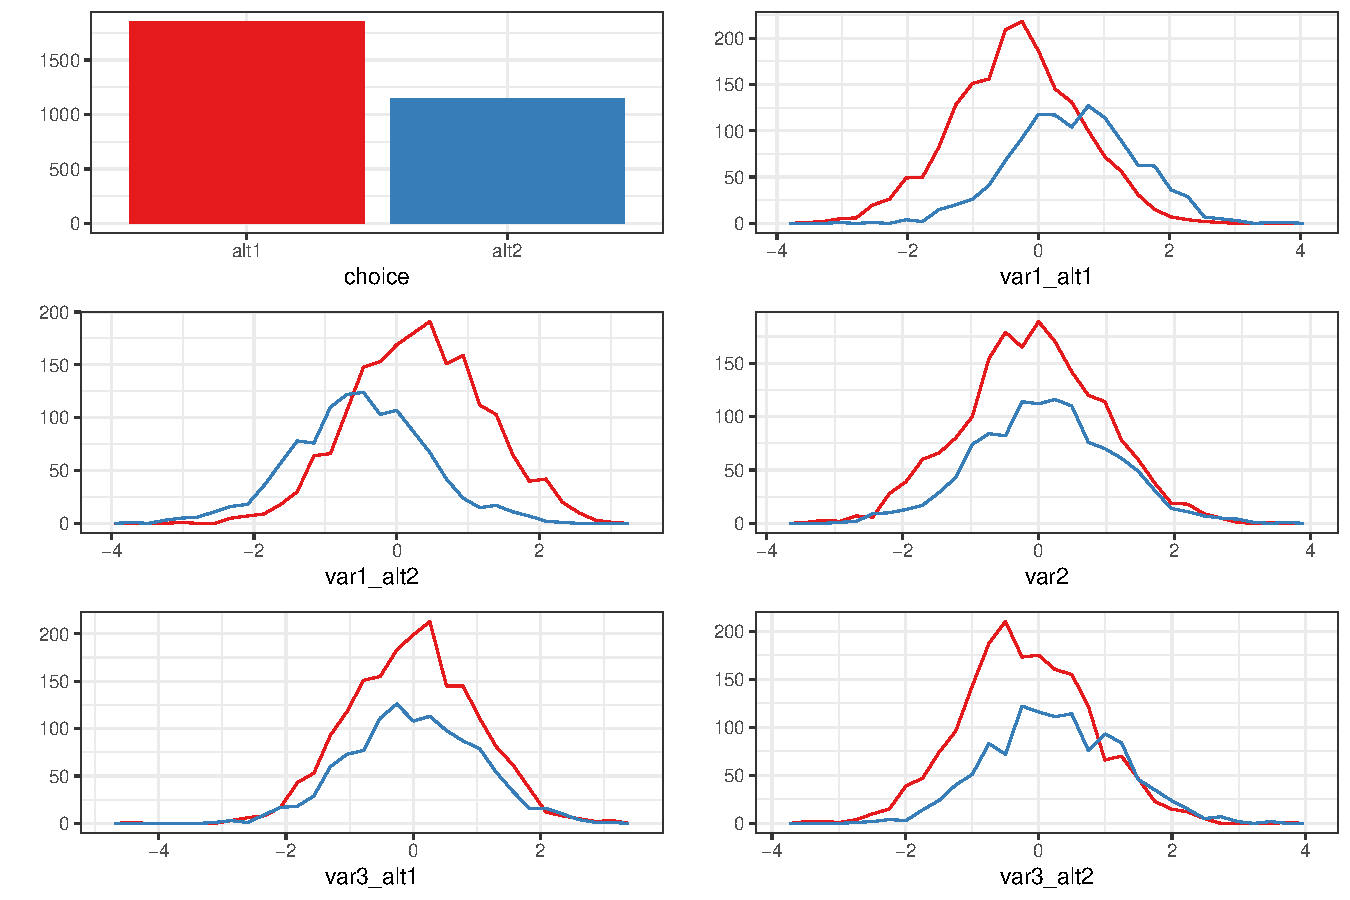
\includegraphics{rprobitb_oelschlaeger_bauer-sim-data}

The graphic is consistent with our model specification: for example, covariate \code{var1} was specified to have a negative effect on \code{alt1}, because the coefficient of \code{var1} (the first value of \code{alpha}) is negative $(-2)$. Hence, higher values of \code{var1\_alt1} correspond more frequently to choice \code{alt2} (top right panel).

\section{Model fitting} \label{sec:model_fitting}

\pkg{RprobitB} estimates the probit model in a Bayesian framework that builds upon the work of \cite{McCulloch:1994}, \cite{Nobile:1998}, \cite{Allenby:1998}, and \cite{Imai:2005}. A key ingredient is the concept of data augmentation \citep{Albert:1993}, which treats the latent utilities in Equation~\ref{eq:utility} as additional parameters. Then, conditional on these parameters, the probit model constitutes a standard Bayesian linear regression setup. Its posterior distribution can be approximated via Gibbs sampling.

\subsection{Prior and posterior distributions} \label{subsec:prior_and_posterior}

We a priori assume the following (conjugate) parameter distributions:
\begin{itemize}
  \item $(s_1,\dots,s_C)\sim D_C(\delta)$, where $D_C(\delta)$ denotes the $C$-dimensional Dirichlet distribution with concentration parameter vector $\delta = (\delta_1,\dots,\delta_C)$,
  \item $\alpha\sim \text{MVN}_{P_f}(\psi,\Psi)$, where $\text{MVN}_{P_f}$ denotes the $P_f$-dimensional normal distribution with mean $\psi$ and covariance $\Psi$,
  \item $b_c \sim \text{MVN}_{P_r}(\xi,\Xi)$, independent for all $c$,
  \item $\Omega_c \sim W^{-1}_{P_r}(\nu,\Theta)$, independent for all $c$, where $W^{-1}_{P_r}(\nu,\Theta)$ denotes the $P_r$-dimensional inverse Wishart distribution with $\nu$ degrees of freedom and scale matrix $\Theta$,
  \item $\tilde{\Sigma} \sim W^{-1}_{J-1}(\kappa,\Lambda)$,
  \item and $d \sim MVN_{J-2}(\zeta,Z)$.
\end{itemize}

These priors imply the following conditional posteriors \citep{Oelschlaeger:2020}:
\begin{itemize}
  \item The class weights are drawn from the Dirichlet distribution
  %
  \begin{align*}
  (s_1,\dots,s_C)\mid \delta,z \sim D_C(\delta_1+m_1,\dots,\delta_C+m_C),
  \end{align*}
  %
  where $m_c=\#\{n:z_n=c\}$ denotes the current absolute size of class $c$. The model is invariant to permutations of the class labels $1,\dots,C$. We therefore accept an update only if the ordering $s_1>\dots>s_C$ still holds (thereby ensuring a unique class labeling).
  \item The allocation variables $(z_n)_n$ are updated independently for all $n$ via
  %
  \begin{align*}
  \text{Prob}(z_n=c\mid s,\beta,b,\Omega )=\frac{s_c\phi_{P_r}(\beta_n\mid b_c,\Omega_c)}{\sum_c s_c\phi_{P_r}(\beta_n\mid b_c,\Omega_c)}.
  \end{align*}
  %
  \item The class means $(b_c)_c$ are updated independently for all $c$ via
  %
  \begin{align*}
  b_c\mid \Xi,\Omega,\xi,z,\beta \sim\text{MVN}_{P_r}\left( \mu_{b_c}, \Sigma_{b_c}  \right),
  \end{align*}
  %
  $\mu_{b_c}=(\Xi^{-1}+m_c\Omega_c^{-1})^{-1}(\Xi^{-1}\xi +m_c\Omega_c^{-1}\bar{b}_c)$, $\Sigma_{b_c}=(\Xi^{-1}+m_c\Omega_c^{-1})^{-1}$, $\bar{b}_c=m_c^{-1}\sum_{n:z_n=c} \beta_n$.
    \item The class covariance matrices $(\Omega_c)_c$ are updated independently for all $c$ via
  %
  \begin{align*}
  \Omega_c \mid \nu,\Theta,z,\beta,b \sim W^{-1}_{P_r}(\mu_{\Omega_c},\Sigma_{\Omega_c}),
  \end{align*}
  %
  $\mu_{\Omega_c}=\nu+m_c$, $\Sigma_{\Omega_c}=\Theta^{-1} + \sum_{n:z_n=c} (\beta_n-b_c)(\beta_n-b_c)^\top$.
  \item Independently for all $n,t$ and conditionally on the other components, the differenced utility vectors $(\tilde{U}_{nt:})$ follow a $(J-1)$-variate truncated normal distribution, where the truncation points are determined by the choices $y_{nt}$. To sample from a truncated multivariate normal distribution, we apply a sub-Gibbs sampler (analogue to \cite{Geweke:1998}):
  %
  \begin{align*}
  \tilde{U}_{ntj} \mid \tilde{U}_{nt(-j)},y_{nt},\tilde{\Sigma},\tilde{W},\alpha,\tilde{X},\beta
  \sim \mathcal{N}(\mu_{\tilde{U}_{ntj}},\Sigma_{\tilde{U}_{ntj}}) \cdot \begin{cases}
  1(\tilde{U}_{ntj}>\max(\tilde{U}_{nt(-j)},0) ) & \text{if}~ y_{nt}=j\\
  1(\tilde{U}_{ntj}<\max(\tilde{U}_{nt(-j)},0) ) & \text{if}~ y_{nt}\neq j
  \end{cases},
  \end{align*}
  %
  where $\tilde{U}_{nt(-j)}$ denotes the vector $(\tilde{U}_{nt:})$ without the element $\tilde{U}_{ntj}$, $\mathcal{N}$ the univariate normal distribution, $\Sigma_{\tilde{U}_{ntj}} = 1/(\tilde{\Sigma}^{-1})_{jj}$, and
  %
  \begin{align*}
  \mu_{\tilde{U}_{ntj}} = \tilde{W}_{ntj}^\top \alpha + \tilde{X}_{ntj}^\top \beta_n - \Sigma_{\tilde{U}_{ntj}} (\tilde{\Sigma}^{-1})_{j(-j)}   (\tilde{U}_{nt(-j)} - \tilde{W}_{nt(-j)}^\top \alpha - \tilde{X}_{nt(-j)}^\top \beta_n ),
  \end{align*}
  %
  where $(\tilde{\Sigma}^{-1})_{jj}$ denotes the $(j,j)$-th element of $\tilde{\Sigma}^{-1}$, $(\tilde{\Sigma}^{-1})_{j(-j)}$ the $j$-th row without the $j$-th entry, $\tilde{W}_{nt(-j)}$ and $\tilde{X}_{nt(-j)}$ the differenced covariate matrices connected to fixed and random effects, respectively, with the $j$-th column removed.

  In the ordered probit case, the (one-dimensional) utility in each choice occasion is drawn from a truncated normal distribution, where the truncation points are determined by the threshold increments $d$.
  \item Updating the fixed coefficient vector $\alpha$ is achieved by applying the formula for Bayesian linear regression of the regressors $\tilde{W}_{nt}$ on the regressands $(\tilde{U}_{nt:})-\tilde{X}_{nt}^\top \beta_n$, i.e.,
  %
  \begin{align*}
  \alpha \mid \Psi,\psi,\tilde{W},\tilde{\Sigma},\tilde{U},\tilde{X},\beta \sim \text{MVN}_{P_f}(\mu_\alpha,\Sigma_\alpha),
  \end{align*}
  %
  $\mu_\alpha = \Sigma_\alpha (\Psi^{-1}\psi + \sum_{n=1,t=1}^{N,T} \tilde{W}_{nt} \tilde{\Sigma}^{-1} ((\tilde{U}_{nt:})-\tilde{X}_{nt}^\top \beta_n) )$, $\Sigma_\alpha = (\Psi^{-1} + \sum_{n=1,t=1}^{N,T} \tilde{W}_{nt}\tilde{\Sigma}^{-1} \tilde{W}_{nt}^\top )^{-1}$.
  \item Analogously to $\alpha$, the random coefficients $(\beta_n)_n$ are updated independently via
  %
  \begin{align*}
  \beta_n \mid \Omega,b,\tilde{X},\tilde{\Sigma},\tilde{U},\tilde{W},\alpha \sim \text{MVN}_{P_r}(\mu_{\beta_n},\Sigma_{\beta_n}),
  \end{align*}
  %
  $\mu_{\beta_n} = \Sigma_{\beta_n} (\Omega_{z_n}^{-1}b_{z_n} + \sum_{t=1}^{T} \tilde{X}_{nt} \tilde{\Sigma}^{-1} ((\tilde{U}_{nt:})-\tilde{W}_{nt}^\top \alpha) )$, $\Sigma_{\beta_n} = (\Omega_{z_n}^{-1} + \sum_{t=1}^{T} \tilde{X}_{nt}\tilde{\Sigma}^{-1} \tilde{X}_{nt}^\top )^{-1}$.
    \item The covariance matrix $\tilde{\Sigma}$ of the error term differences is updated by means of
  %
  \begin{align*}
  \tilde{\Sigma} \mid \kappa,\Lambda,\tilde{U},\tilde{W},\alpha,\tilde{X},\beta \sim W^{-1}_{J-1}(\kappa+NT,\Lambda+S),
  \end{align*}
  %
  where $S = \sum_{n=1,t=1}^{N,T} \tilde{\varepsilon}_{nt} \tilde{\varepsilon}_{nt}^\top$ and $\tilde{\varepsilon}_{nt} = (\tilde{U}_{nt:}) - \tilde{W}_{nt}^\top \alpha - \tilde{X}_{nt}^\top \beta_n$.
  \item The utility thresholds \code{d} are updated by means of a Metropolis–Hastings algorithm with a normal proposal density.
\end{itemize}

The Gibbs samples obtained from this updating scheme (except for $s$ and $z$) lack identification with respect to the scale (cf., Section \ref{sec:probit_model}). Subsequent to the sampling and for the $i$-th updates in each iteration $i$, we therefore apply the normalization $\alpha^{(i)} \cdot \omega^{(i)}$, $b_c^{(i)} \cdot \omega^{(i)}$, $\tilde{U}_{nt}^{(i)} \cdot \omega^{(i)}$, $\beta_n^{(i)} \cdot \omega^{(i)}$, $\Omega_c^{(i)} \cdot (\omega^{(i)})^2$, $\tilde{\Sigma}^{(i)} \cdot (\omega^{(i)})^2$, and $\gamma^{(i)} \cdot \omega^{(i)}$, where either $\omega^{(i)} = (\text{const} / (\tilde{\Sigma}^{(i)})_{jj})^{0.5}$ with $(\tilde{\Sigma}^{(i)})_{jj}$ the $j$-th diagonal element of $\tilde{\Sigma}^{(i)}$, $1\leq j \leq J-1$, or alternatively $\omega^{(i)} = \text{const} / \alpha^{(i)}_p$ for some coordinate $1\leq p \leq P_f$ of the $i$-th draw for the coefficient vector $\alpha$. Here, '$\text{const}$' is a constant to specify custom utility scales.

\subsection{The estimation routine} \label{subsec:estimation_routine}

The Gibbs sampling scheme can be executed via \code{fit\_model(data = data)}, where \code{data} is an \class{RprobitB\_data} object (introduced in Section \ref{sec:choice_data}).\footnote{The \class{RprobitB\_data} object already contains the model formula and the random effect specification.} Optional arguments are:

\begin{itemize}
  \item \code{scale}: A character which determines the utility scale (cf., Section \ref{sec:probit_model}). It is of the form \code{"<parameter> := <value>"}, where \code{<parameter>} is either the name of a fixed effect or \code{Sigma\_<j>,<j>} for the \code{<j>}-th diagonal element of \code{Sigma}, and \code{<value>} is the value of the fixed parameter (i.e., '$\text{const}$' from above). Per default \code{scale = "Sigma\_1,1 := 1"}, i.e., the first error term variance is fixed to 1.
  \item \code{R}: The number of iterations of the Gibbs sampler. The default is \code{R = 1000}.
  \item \code{B}: The length of the burn-in period (\code{B = R/2} by default).\footnote{The theory behind Gibbs sampling constitutes that the sequence of samples produced by the
updating scheme is a Markov chain with stationary distribution equal to the desired joint posterior distribution. It takes a certain number of iterations for that stationary distribution to be approximated reasonably well. Therefore, it is common practice to discard the first \code{B} out of \code{R} samples (the so-called burn-in period).}
  \item \code{Q}: The thinning factor for the Gibbs samples (\code{Q = 1} by default).
  \item \code{print\_progress}: A boolean, determining whether to print the Gibbs sampler progress.
  \item \code{prior}: A named list of parameters for the prior distributions. Default values are documented in the \fct{check\_prior} function, see \code{help(check\_prior, package = "RprobitB")}.
\end{itemize}

\paragraph{Example 1: Train trips (cont.).}

Recall the \code{Train} data set of stated train trip alternatives, characterized by their \code{price}, \code{time}, number of \code{change}s, and level of \code{comfort}. From this data, we previously built the \class{RprobitB\_data} object \code{data\_train}, which we now pass to the estimation routine. For scale normalization, we fix the \code{price} coefficient to \code{-1}, which has the advantage that we can interpret the other coefficients as monetary values:

\begin{Schunk}
\begin{Sinput}
> model_train <- fit_model(data = data_train, scale = "price := -1")
\end{Sinput}
\end{Schunk}

We can visualize the estimated coefficients (the Gibbs sample means) as follows:

\begin{Schunk}
\begin{Sinput}
> plot(coef(model_train), sd = 3)
\end{Sinput}
\end{Schunk}
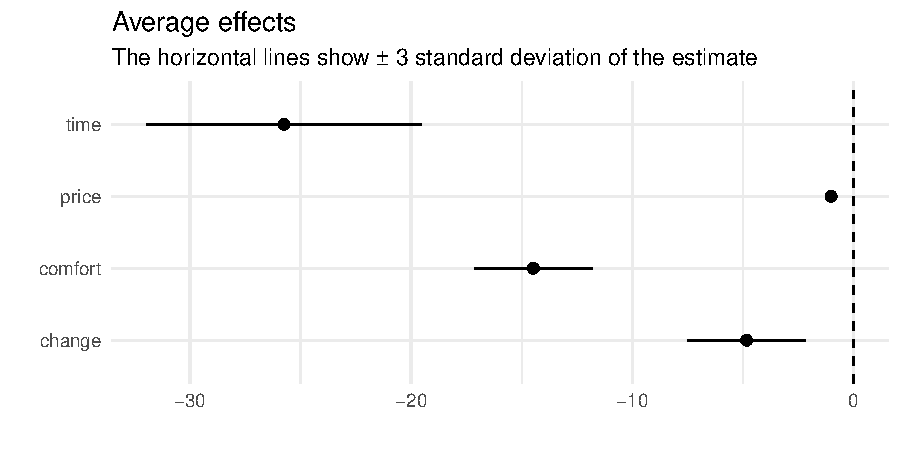
\includegraphics{rprobitb_oelschlaeger_bauer-coef-model-train}

The results indicate that the deciders value one hour travel time by about 26 euros, an additional change by 5 euros, and a more comfortable class by 14 euros.\footnote{We note that these results are consistent with the ones that are presented in a vignette of \pkg{mlogit} entitled "The random parameters (or mixed) logit model" on the same data set but using the logit model.} Calling the \fct{summary} method on the estimated \class{RprobitB\_fit} object yields additional information about the (transformed) Gibbs samples. The method receives a list \code{FUN} of arbitrary functions that can compute point estimates of the Gibbs samples, by default \fct{mean} for the arithmetic mean, \fct{stats::sd} for the standard deviation, and \fct{R\_hat} for the Gelman-Rubin statistic\footnote{A Gelman-Rubin statistic (a lot) greater than 1 indicates convergence issues of the Gibbs sampler.} \citep{Gelman:1992}:

\begin{Schunk}
\begin{Sinput}
> summary(model_train, FUN = c("mean" = mean, "sd" = stats::sd, "R^" = R_hat))
\end{Sinput}
\begin{Soutput}
Probit model
Formula: choice ~ price + time + comfort + change | 0 
R: 1000, B: 500, Q: 1
Level: Utility differences with respect to alternative 'B'.
Scale: Coefficient of effect 'price' (alpha_1) fixed to -1.

Gibbs sample statistics
          mean      sd      R^
 alpha
                              
     1   -1.00    0.00    1.00
     2  -25.89    2.28    1.00
     3  -14.44    0.90    1.00
     4   -4.91    0.89    1.01

 Sigma
                              
   1,1  656.92   63.81    1.04
\end{Soutput}
\end{Schunk}

The \fct{plot} method with the additional argument \code{type = "trace"} visualizes the trace of the transformed and thinned Gibbs samples after the burn-in period:

\begin{Schunk}
\begin{Sinput}
> par(mfrow = c(1,2))
> plot(model_train, type = "trace")
\end{Sinput}
\end{Schunk}
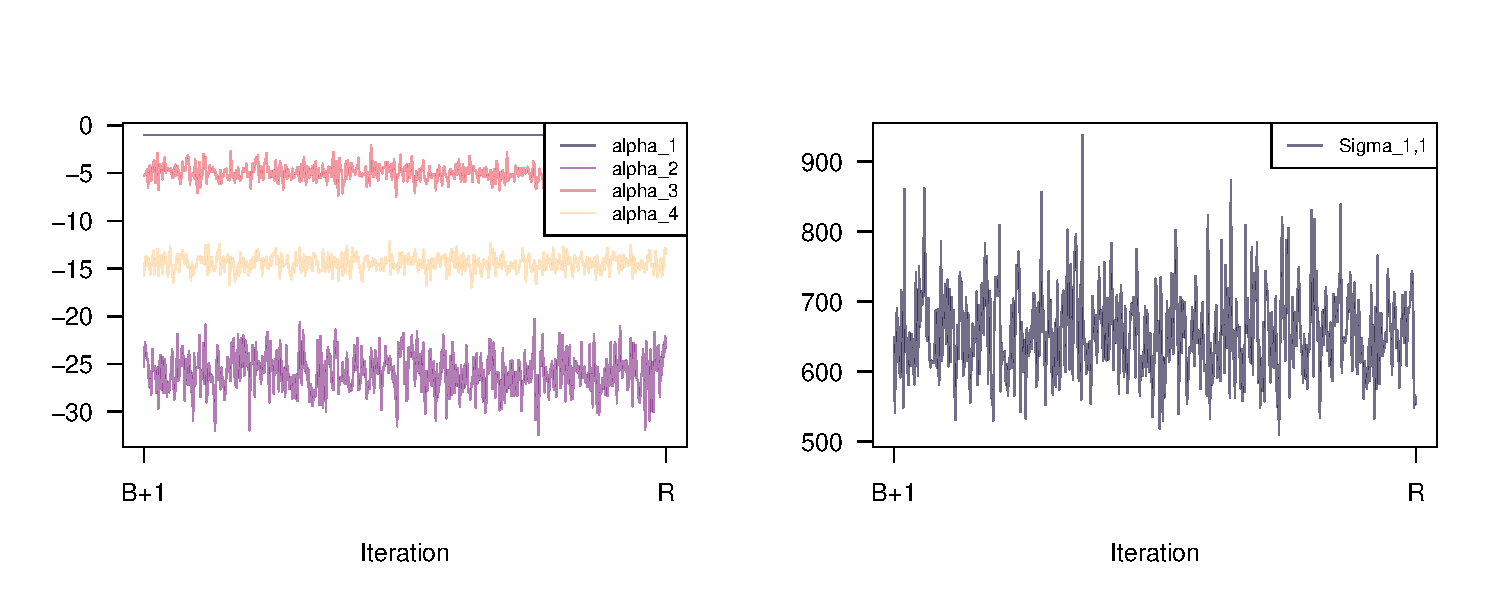
\includegraphics{rprobitb_oelschlaeger_bauer-model-train-trace}

Additionally, we can plot the autocorrelation of the Gibbs samples via \code{type = "acf"}, below exemplary for \code{alpha\_4} and \code{Sigma\_1,1}. The boxes in the plot's top right corner state the total sample size TSS, given by (\code{R} - \code{B}) / \code{Q}, and the effective sample size ESS. The effective sample size is the value $\text{TSS} \cdot \sigma^2 / f(0)$, where $f(0) = \sigma^2(1 + 2\sum_{k\geq 1} \rho_k)$ denotes the spectrum at frequency zero of the stationary output of the Gibbs sampler \citep{Marin:2014}. The spectrum is estimated via the \fct{stats::spec.ar} function.

\begin{Schunk}
\begin{Sinput}
> par(mfrow = c(1,2))
> plot(model_train, type = "acf", ignore = c("alpha_1", "alpha_2", "alpha_3"))
\end{Sinput}
\end{Schunk}
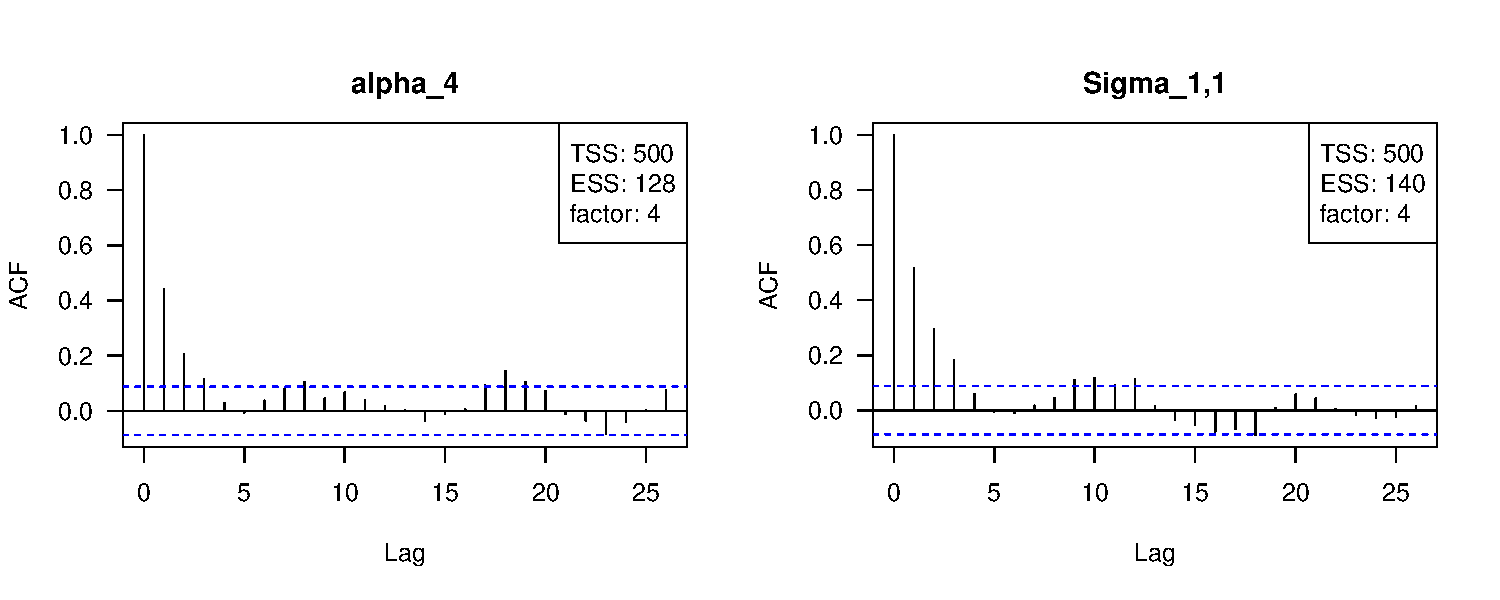
\includegraphics{rprobitb_oelschlaeger_bauer-model-train-acf}

The \fct{transform} method can be used to reduce the autocorrelation in a subsample (commonly referred to as "thinning"):\footnote{The function can also be used to change the length of the burn-in period with \code{transform(model\_train, B = B\_new)} or the utility scale, e.g., \code{transform(model\_train, scale = "Sigma\_1,1 := 1")}.}

\begin{Schunk}
\begin{Sinput}
> model_train <- transform(model_train, Q = 5)
\end{Sinput}
\end{Schunk}

\paragraph{Example 3: Electricity suppliers.}

The \code{Electricity} data set from \pkg{mlogit} contains choices of residential electricity customers that decide between four hypothetical electricity suppliers. We expect heterogeneity in choice behavior here, because customers might value certain contract characteristics differently based on their living conditions. In particular, the contracts differed in six characteristics: their fixed price \code{pf} per kilowatt hour, their contract length \code{cf}, whether the supplier is a local company (\code{loc}), whether the supplier is a well known company (\code{wk}), whether the supplier offers a time-of-day electricity price which is higher during the day and lower during the night (\code{tod}), and whether the supplier's price is seasonal dependent (\code{seas}).

The following lines prepare the data set for estimation. We first use the convenience function \fct{as\_cov\_names} that relabels the data columns for alternative specific covariates into the required format \code{"<covariate>\_<alternative>"}:

\begin{Schunk}
\begin{Sinput}
> data("Electricity", package = "mlogit")
> Electricity <- as_cov_names(
+    choice_data = Electricity, cov = c("pf","cl","loc","wk","tod","seas"),
+    alternatives = 1:4
+  )
\end{Sinput}
\end{Schunk}

Via the \code{re = c("cl","loc","wk","tod","seas")} argument, we specify random effects for all but the price coefficient, which we again fix to \code{-1} for monetary interpretation:

\begin{Schunk}
\begin{Sinput}
> data_elec <- prepare_data(
+    form = choice ~ pf + cl + loc + wk + tod + seas | 0,
+    choice_data = Electricity,
+    re = c("cl","loc","wk","tod","seas")
+  )
> model_elec <- fit_model(data_elec, scale = "pf := -1")
\end{Sinput}
\end{Schunk}

The \fct{coef} method returns the average effects and the estimated (marginal) variances:

\begin{Schunk}
\begin{Sinput}
> coef(model_elec)
\end{Sinput}
\begin{Soutput}
        Estimate   (sd) Variance   (sd)
1   pf     -1.00 (0.00)       NA   (NA)
2   cl     -0.26 (0.03)     0.36 (0.06)
3  loc      2.88 (0.26)     7.20 (1.24)
4   wk      2.10 (0.21)     4.01 (0.75)
5  tod     -9.85 (0.24)    12.15 (2.01)
6 seas     -9.90 (0.19)     6.26 (0.95)
\end{Soutput}
\end{Schunk}

We deduce, for example, that a longer contract length has a negative effect on average (-0.26). However, our model shows that 33\% of the customers still prefer to have a longer contract length. This share is estimated by computing the proportion under the mixing distribution that yields a positive coefficient for \code{cl}:

\begin{Schunk}
\begin{Sinput}
> cl_mu <- coef(model_elec)["cl","mean"]
> cl_sd <- sqrt(coef(model_elec)["cl","var"])
> pnorm(cl_mu / cl_sd)
\end{Sinput}
\begin{Soutput}
[1] 0.3316322
\end{Soutput}
\end{Schunk}

The estimated joint mixing distribution additionally allows to infer correlation patterns between effects. For example, we find a correlation of 0.79 between \code{loc} and \code{wk} (deciders that prefer local suppliers also prefer well known companies):

\begin{Schunk}
\begin{Sinput}
> round(cov_mix(model_elec, cor = TRUE), 2)
\end{Sinput}
\begin{Soutput}
        cl   loc    wk   tod  seas
cl    1.00  0.09  0.06 -0.05 -0.11
loc   0.09  1.00  0.79  0.08 -0.01
wk    0.06  0.79  1.00  0.09 -0.03
tod  -0.05  0.08  0.09  1.00  0.55
seas -0.11 -0.01 -0.03  0.55  1.00
\end{Soutput}
\end{Schunk}

\paragraph{Example 2: Simulated choices (cont.).}

We previously simulated the \class{RprobitB\_data} object \code{data\_sim} from a probit model with three latent classes. We now estimate the model parameters from the data generating process:

\begin{Schunk}
\begin{Sinput}
> model_sim <- fit_model(
+    data = data_sim, R = 1000, latent_classes = list("C" = 3), seed = 1
+  )
> summary(model_sim)
\end{Sinput}
\begin{Soutput}
Probit model
Formula: choice ~ var1 | var2 | var3 
R: 1000, B: 500, Q: 1
Level: Utility differences with respect to alternative 'alt2'.
Scale: Coefficient of the 1. error term variance fixed to 1.

Latent classes
C = 3 

Gibbs sample statistics
          true    mean      sd      R^
 alpha
                                      
     1   -2.00   -2.00    0.13    1.21
     2    0.00   -0.04    0.03    1.10
     3    1.00    0.99    0.08    1.18

 s
                                      
     1    0.60    0.63    0.06    1.33
     2    0.30    0.27    0.06    1.10
     3    0.10    0.10    0.04    1.13

 b
                                      
   1.1   -2.00   -1.90    0.13    1.05
   1.2    1.00    0.93    0.23    1.70
   2.1    0.00    0.01    0.31    1.43
   2.2    2.00    2.04    0.36    1.40
   3.1    2.00    2.13    0.72    1.04
   3.2   -1.00   -0.84    0.83    1.06

 Omega
                                      
 1.1,1    0.30    0.61    0.22    1.82
 1.1,2    0.70    0.72    0.27    1.85
 1.2,2    1.90    2.11    0.52    1.68
 2.1,1    1.30    1.20    0.52    1.03
 2.1,2   -0.20   -0.25    0.31    1.00
 2.2,2    0.90    1.02    0.37    1.26
 3.1,1    0.60    1.66    1.43    1.05
 3.1,2   -0.90   -0.79    1.44    1.03
 3.2,2    2.40    2.82    1.46    1.03

 Sigma
                                      
   1,1    1.00    1.00    0.00    1.00
\end{Soutput}
\end{Schunk}

We note that more than $R = 1000$ iterations are required for proper convergence, as indicated by the Gelman-Rubin statistic.

\subsection{Weight-based update of latent classes} \label{subsec:weight_update}

Adding \code{"weight_update" = TRUE} to the list for the \code{latent\_classes} argument of \fct{fit\_model} executes the following weight-based updating scheme of the latent classes:

\begin{itemize}
  \item Class $c$ is removed, if $s_c<\varepsilon_{\text{min}}$, i.e., if the class weight $s_c$ drops below some threshold $\varepsilon_{\text{min}}$. This case indicates that class $c$ has a negligible impact on the mixing distribution.
  \item Class $c$ is split into two classes $c_1$ and $c_2$, if $s_c>\varepsilon_\text{max}$. This case indicates that class $c$ has a high influence on the mixing distribution whose approximation can potentially be improved by increasing the resolution in directions of high variance. Therefore, the class means $b_{c_1}$ and $b_{c_2}$ of the new classes $c_1$ and $c_2$ are shifted in opposite directions from the class mean $b_c$ of the old class $c$ in the direction of the largest diagonal element of the class covariance matrix $\Omega_c$.
  \item Classes $c_1$ and $c_2$ are joined to one class $c$, if $\lVert b_{c_1} - b_{c_2} \rVert<\varepsilon_{\text{distmin}}$, i.e., if the euclidean distance between the class means $b_{c_1}$ and $b_{c_2}$  drops below some threshold $\varepsilon_{\text{distmin}}$. This case indicates location redundancy which should be repealed. The parameters of the new class $c$ are assigned by adding the values of $s$ from $c_1$ and $c_2$ and averaging the values for $b$ and $\Omega$.
\end{itemize}

The values for $\varepsilon_{\text{min}}$, $\varepsilon_{\text{max}}$ and $\varepsilon_{\text{distmin}}$ can be specified via the \code{latent\_classes} argument (by default \code{epsmin = 0.01}, \code{epsmax = 0.99}, and \code{distmin = 0.1}).

\paragraph{Example 2: Simulated choices (cont.).}

We apply the weight-based updating scheme to reproduce the true number $C = 3$ of latent classes. The scheme is initialized with \code{"C" = 10} classes and executed every \code{"buffer" = 5}-th iteration:

\begin{Schunk}
\begin{Sinput}
> model_sim <- fit_model(
+    data = data_sim, seed = 1,
+    latent_classes = list("C" = 10, "weight_update" = TRUE, "buffer" = 5)
+  )